%!TEX root = /Users/andy/Documents/Academics/Dissertation/thesis.tex

\chapter{Bending waves during \textit{Caenorhabditis elegans} locomotion are driven and organized by proprioceptive coupling }


\section{Introduction}
\lettrine{H}{ow neural circuits give rise to coordinated rhythmic behaviors} such as locomotion remains a fundamental question in systems neuroscience 
\citep{delcomyn_neural_1980}. Classic studies sought the neuromuscular 
basis of locomotion in aquatic swimmers such as lamprey and leech \citep{marder_principles_1996,kristan_rhythmic_1976,cohen_neuronal_1980,friesen_neuronal_1978,ermentrout_frequency_1984}. In these systems, the concept of a Central Pattern Generator (CPG) is commonly evoked to explain rhythmic behavior \citep{delcomyn_neural_1980,marder_principles_1996}. The CPG hypothesis is supported by observations that motor neurons in each body segment continue to exhibit rhythmic activity even after pruning all inputs \citep{kristan_rhythmic_1976,cohen_neuronal_1980,pearce_intersegmental_1984}.




Whereas a CPG could produce rhythmic behavior, motor circuits still need to respond to sensory 
inputs to deliver precise and flexible control of body movement \citep{delcomyn_neural_1980}. In leech, muscle activity can be coordinated among segments by sensory feedback even after cutting neuronal couplings between segments \citep{yu_sensory_1999}. In \textit{Drosophila larva}, specific classes of mechanosensory neurons that tile the whole body contribute to organizing peristaltic waves during locomotion \citep{hughes_sensory_2007,song_peripheral_2007,cheng_role_2010}. In \textit{C. 
elegans}, the shape and speed of bending waves adapt to the mechanical load imposed by the 
environment \citep{fang-yen_biomechanical_2010,berri_forward_2009}, and mutations in a mechanosensitive channel (TRP-4) acting in the DVA 
interneuron perturb the amplitude and frequency of body undulation \citep{li_c._2006}.


Here, we sought a biophysical characterization of the role of proprioceptive feedback in the \textit{C. elegans} locomotory circuit by combining microfluidics and optical neurophysiology \citep{liewald_optogenetic_2008,chronis_microfluidics_2007,zhang_multimodal_2007,clark_temporal_2007,lockery_artificial_2008}. We discovered that stretch-sensitive coupling between adjacent body regions represents the key mechanism for driving bending waves along the worm body during forward locomotion.





\section{Results}
\subsection{The bending of one body region requires the bending of its anterior neighbor}

\textit{C. elegans} moves forward by propagating dorsal-ventral body bending waves from head to tail. 
The detailed kinematics of bending waves can be quantified using the time-varying curvature 
measured at each point along the body centerline over time (Fig.~\ref{fig:proc1}a). To compare data from different worms, we normalized distance along the centerline by measuring fractional distance 
from head to tail (head $=0$; tail $=1$). Each body region alternates between positive (red) and 
negative (blue) curvature and bands of curvature propagate from head to tail as shown in a 
kymograph (Fig.~\ref{fig:proc1}b). 




\begin{FPfigure} 
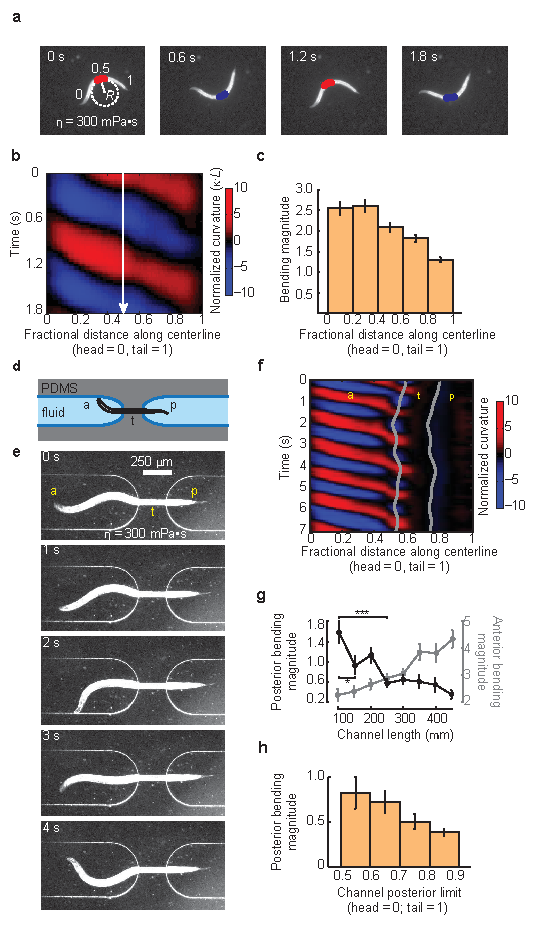
\includegraphics[width=\textwidth]{figures/proc1}
\caption[Bending of posterior regions requires anterior bending. ] {Bending of posterior regions requires anterior bending. (\textbf{a}) Video images of a worm swimming forward. Bending is quantified by measuring the radius 	of curvature R at each point along the centerline. Position along the centerline is measured in normalized coordinates using the fractional distance from head to tail (head $= 0$; tail $= 1$). A red-blue colormap illustrates alternating curvatures at fractional distance $= 0.5$. (\textbf{b}) Kymograph of time-varying curvature illustrating retrograde bending waves along the worm represented in non-dimensional units. To do this, the curvature at each point along the centerline, $\kappa = 1/R$, is multiplied by worm length, $L$. (\textbf{c}) Bending magnitude along the body of a wide-type free swimming worm, measured as the standard deviation of normalized curvature over time. $n = 18$ worms, mean $\pm$ one standard error. (\textbf{d}) Schematic of microfluidic device. a stands for anterior region, p stands for posterior region, and t stands for trapped region of a worm.  (\textbf{e}) Video images of a wide-type young adult worm exhibiting forward undulatory gait inside the microfluidic device (also see Supplementary Movie 1). The channel divides the worm body into unrestrained anterior, posterior, and trapped middle regions. (\textbf{f}) Kymograph of time-varying curvature along the body of the worm shown in (\textbf{e}). Gray lines mark the anterior and posterior limits of the straight channel. (\textbf{g}) Bending magnitude of a posterior and an anterior body region (\textasciitilde$0.15$ worm length) adjacent to the channel, measured as the standard deviation of time-varying normalized curvature, is plotted as a function of the length of the trapped region. $n \geq 10$ worms for each condition, mean  $15$	$\pm$ one standard error. Position of the posterior limit of the channel is $0.7 \pm 0.1$ (mean $\pm$ standard deviation) for each condition, measured as the fractional distance from head to tail. *$P<0.05$, ***$P = 0.0001$, Mann-Whitney U test.  (\textbf{h}) Bending magnitude of a posterior body region (mean $\pm$ one standard error) as a function of the position of the posterior limit of the channel. We measured 64 bouts of forward movement trapped in different channel positions from $20$ worms. Channel length is $300 \mu$m.\label{fig:proc1}}
\end{FPfigure}



First, we sought to determine whether the motor activity in one body region might depend on the 
bending of neighboring body regions. To test this, we designed microfluidic devices that enabled 
us to immobilize body regions of varying length along the middle of a young adult worm (Fig.~\ref{fig:proc1}d-e and Supplementary Movie 1). Our first device trapped the center of a worm in a narrow 
straight channel. The region of the worm's body inside the channel was restrained, while  regions of the worm's body either anterior or 
posterior to the channel were free to bend (Fig.~\ref{fig:proc1}d-e). We used a channel diameter ($40 \mu$m) that was sufficient to 
immobilize the trapped region (worm diameter is $54 \pm 4 \mu$m; mean $\pm$ SD) with minimum 
constriction.  

We consistently recorded bouts of forward movement ($> 10$ s) when we set the posterior limit of 
the channel at $0.7 \pm 0.1$ in fractional worm length along the body. Bending waves would 
propagate normally to the anterior limit of the channel (gray data points in Fig.~\ref{fig:proc1}g). Short 
channels ($100 \mu$m long) did not affect wave propagation along the worm body; the bending wave 
that emerged from the posterior limit of the channel (black data points in Fig.~\ref{fig:proc1}g) exhibited 
similar amplitude as a free swimming worm (Fig.~\ref{fig:proc1}c). However, increasing channel length 
beyond $200 \mu$m significantly diminished the bending amplitude in the posterior body region (Fig.~\ref{fig:proc1}e-g). Fixing the channel length, but moving it towards the tail also reduced the posterior 
bending amplitude (Fig.~\ref{fig:proc1}h, $R = -0.24$, $p < 0.05$, Spearman’s rank correlation test).

To determine whether immobilization directly affects muscle activity in body regions within and 
posterior to the channel, we quantified intracellular calcium dynamics in the muscle cells of 
transgenic worms (P\textit{myo3::G-CaMP3::RFP}) expressing the calcium indicator G-CaMP3 \citep{tian_imaging_2009} and RFP in all body wall muscles (Supplementary Fig.~\ref{fig:procSup2} and Supplementary Movie 2). While 
muscle cells anterior to the channel exhibited strong rhythmic intracellular calcium dynamics 
during the propagation of bending waves, muscle cells within and posterior to the channel had 
much lower levels of calcium dynamics (Supplementary Fig.~\ref{fig:procSup2}).

Taken together, these results suggest that immobilizing a body region lowers motor activity 
within and posterior to that region, thereby disrupting bending wave propagation. Motor activity 
in one body region seems to require the active bending of anterior regions extending \textasciitilde200 $\mu$m.

\subsection{Muscle activity is positively correlated with the curvature of adjacent anterior 
neighbors}
 
To further explore how the bending of adjacent body regions is coupled, we designed 
microfluidic devices that trapped a middle region of a worm at defined curvatures (Fig.~\ref{fig:proc2}a,c). 
Here, we used channels that were at least $250 \mu$m long to prevent bending waves from 
propagating into the unrestrained posterior part. The unrestrained posterior region exhibited 
static curvature in the same direction as that imposed on the middle region trapped by the 
channel (Fig.~\ref{fig:proc2}a-b and Supplementary Movie 3). By using channels with different curvatures, we 
found that the curvature of the posterior region increased linearly with the imposed curvature on 
the trapped middle region with slope $0.62 \pm 0.03 L$ (Fig.~\ref{fig:proc2}d). 



\begin{FPfigure} 
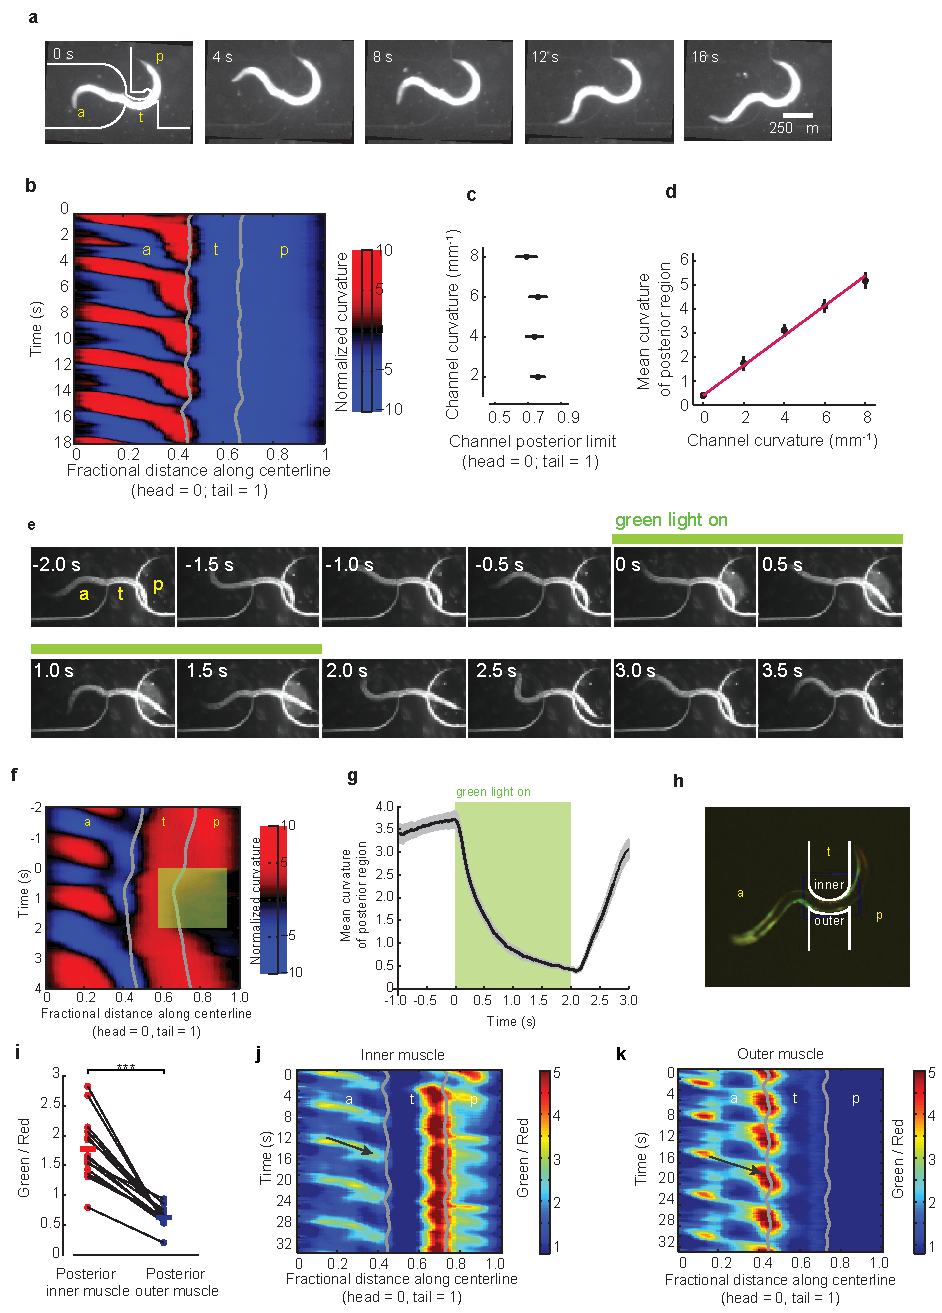
\includegraphics[width=\textwidth]{figures/proc2}
\caption[Bending of posterior regions is positively correlated with anterior bending. ] {Bending of posterior regions is positively correlated with anterior bending. (\textbf{a}) Video images of a worm exhibiting forward undulatory gait while partially constrained in a 
curved microfluidic channel (also see Supplementary Movie 3). 
(\textbf{b}) Kymograph of normalized curvature of the worm shown in (\textbf{a}). Gray lines show anterior and 
posterior limits of the curved channel. 
(\textbf{c}) Positions of the posterior limit of the curved channel (mean $\pm$ standard deviation). $n \geq 8$ 
worms for each condition,  
(\textbf{d}) The curvature of the unrestrained posterior body region, measured as a spatial average from 
the posterior limit of the channel to the tail and a temporal average over bouts of forward 
movement, is plotted as a function of channel curvature. Each data point (mean $\pm$ one standard 
error) represents data from at least 8 animals. Magenta line is the linear least square fit of the 
data with a slope $0.62 \pm 0.03~L$.  
(\textbf{e}) Video images of a transgenic worm (P\textit{myo3::NpHR}) partially constrained in a curved 
microfluidic channel. The green bar indicates a $2$ s interval during which the posterior body 
region emerging from the channel was illuminated by green light (also see Supplementary Movie 
4). 
(\textbf{f}) Kymograph of normalized curvature of the animal shown in (\textbf{e}). Green shading indicates the 
body region and duration of green light illumination.  
(\textbf{g}) Mean curvature $\pm$ one standard error of the posterior region emerging from the curved 
channels as shown in (\textbf{a}) during green light illumination (\textasciitilde$30$ measurements using 6 worms). 
(\textbf{h}) Calcium imaging of body wall muscles in a partially constrained transgenic worm 
(P\textit{myo3::G-CaMP3::RFP}) in a curved channel. Red fluorescence from RFP constitutes the 
reference signal. Green fluorescence from G-CaMP3 indicates intracellular calcium levels. The 
contours of the microfluidic channel are drawn in white (also see Supplementary Movie 5). 
(\textbf{i}) Comparison of the ratio of green fluorescence to red fluorescence intensity emitted from inner 
and outer muscles of the posterior body region. Each data point represents a spatial average of 
the ratio over a posterior body region (\textasciitilde$0.2$ worm length) adjacent to the channel and a temporal 
average over a bout of forward movement. Solid lines indicate population mean. Among $14$ 
measurements from six worms, six measurements restrict dorsal muscles on the inner side. ***$P= 0.00001$, Mann-Whitney U test. 
(\textbf{j,k}) Representative ratiometric kymograph of calcium levels in inner (\textbf{j}) and outer (\textbf{k}) muscle 
cells of a worm trapped in the device shown in (\textbf{h}). Higher/lower ratios of green fluorescence to 
red fluorescence in each set of body wall muscles indicate higher/lower intracellular calcium 
levels. Arrows highlight one calcium wave that propagates from the head to the anterior limit of 
the curved channel along the inner musculature (\textbf{j}) and outer musculature (\textbf{k}).\label{fig:proc2}}
\end{FPfigure}


We sought to verify that the static curvature of the posterior unrestrained region was driven by 
muscle activity, and not through passive mechanical properties of the worm body. First, we used 
transgenic worms (\textit{Pmyo3::NpHR}) that express halorhodopsin \citep{han_multiple-color_2007} in all body wall muscles. 
When we induced muscle relaxation in the unrestrained posterior region with green light, we 
found that the tail reversibly straightened during illumination (Fig.~\ref{fig:proc2}e-g and Supplementary 
Movie 4). Second, we directly monitored muscle activity in the curved posterior region using 
 $5$
transgenic worms (P\textit{myo3::G-CaMP3::RFP}) that expressed both G-CaMP3 and RFP in all body 
wall muscle cells (Fig.~\ref{fig:proc2}h). Using this strain, intracellular calcium levels within a cell can be 
inferred from the ratio of green to red fluorescence (the higher the ratio, the higher the 
intracellular calcium concentration). In the posterior region emerging from the channel, we 
consistently measured higher calcium levels in the muscle cells on the inner side than the outer 
side of the curved body (Fig.~\ref{fig:proc2}i-k). Third, when the whole animal was paralyzed with sodium 
azide, the body regions emerging from the curved channel remained straight (Supplementary 
Movie 6). These experiments suggest that the static curvature of the posterior unrestrained region 
is due to a fixed pattern of motor circuit activity. 


Taken together, our results suggest that proprioceptive coupling contributes to propagating the 
bending signal along the worm body during forward movement. Through positive stretch- 
sensitive feedback, posterior regions are compelled to bend in the same direction and in 
proportion to the bending of adjacent anterior regions. 
 
\subsection{Post-channel body curvature follows channel curvature with a viscosity- 
dependent delay}
 
To characterize the temporal dynamics of proprioceptive coupling, we measured the time lag 
between the bending in one body region and the induced bending in the neighboring posterior 
region. To do this, we designed pneumatic microfluidic devices to rapidly change the curvature 
of one region of a worm. We flanked both sides of a thin channel with two independently 
controllable inflatable chambers (Fig.~\ref{fig:proc3}a). By simultaneously pressurizing one chamber while 
depressurizing the other, we were able to induce rapid curvature changes in a specific region of a 
trapped worm. 

\begin{FPfigure} 
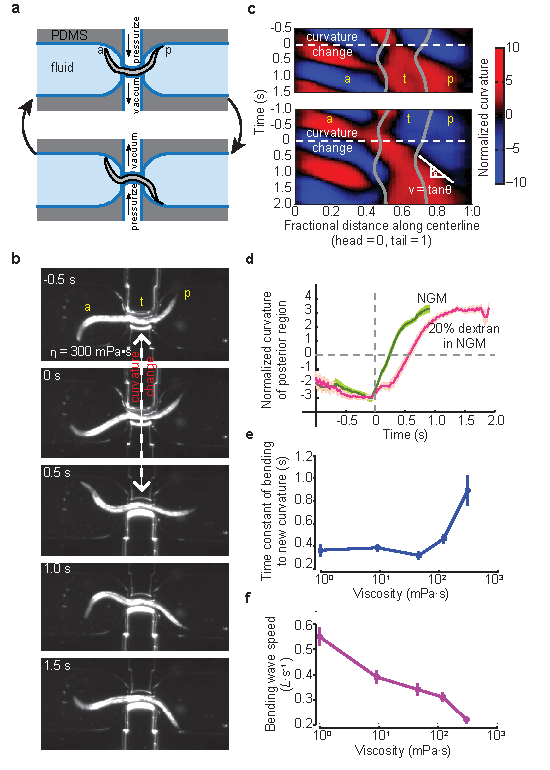
\includegraphics[width=\textwidth]{figures/proc3}
\caption[Pneumatic microfluidic device for manipulating body curvature.] {Pneumatic microfluidic device for manipulating body curvature.  
(\textbf{a}) Schematic of the pneumatic microfluidic device. The channel is flanked by two chambers. By 
alternatively pressurizing one chamber while depressurizing the other, the curvature of a region 
of a trapped worm is rapidly switched. 
(\textbf{b}) Video images of a partially immobilized wild-type worm. At $t = 0$ s, the channel starts to 
change its curvature (also see Supplementary Movie 7). 
(\textbf{c}) Two representative curvature kymographs of a worm trapped in the pneumatic channel. Gray 
lines mark the anterior and posterior limits of the curved channels. White dashed lines at $t = 0$ s 
mark the induced change in channel curvature from negative (color blue) to positive (color red). 
While the unrestricted anterior body region exhibits opposite bending activities in the two 
kymographs, this difference did not affect the dynamics of the induced curvature change in the 
unrestricted posterior body region. The bending wave that shifts the posterior region from 
negative to positive curvature propagates with velocity equal to the slope of the zero crossing in 
curvature (color black) as shown. 

(\textbf{d}) The time course of curvature change in the immediate posterior region (\textasciitilde$0.1$ worm length) 
emerging from the pneumatic channel after the switch of channel curvature at $t = 0$ s. The two 
curves correspond to experiments conducted in two different viscosities (NGM buffer and $20\%$ 
dextran in NGM). Error bars indicate one standard error.  
(\textbf{e}) The time constant for relaxation of the posterior region to new curvatures obtained by fitting 
exponentials to time courses as shown in (\textbf{d}). Each data point represents at least $30$ 
measurements from five worms. Error bars indicate $95\%$ confidence interval to the exponential 
fits.  
(\textbf{f}) The speed of the bending wave following induced changes in channel curvature as a function 
of fluid viscosity. Error bars indicate one standard error.\label{fig:proc3}}
\end{FPfigure}


As with the static curved channels, we found that the curvature of the worm body posterior to the 
dynamic channel was positively correlated with channel curvature. Switching channel curvature 
to either side induced a switch in the curvature of the posterior body region (Fig.~\ref{fig:proc3}b-c and 
Supplementary Movie 7). This result also underscores dorsal/ventral symmetry in the coupling 
mechanism between adjacent body regions. 

We found that the switch in curvature of the posterior unrestrained region propagated with 
measurable speed from the posterior limit of the channel to the tail, consistent with the flow of a 
retrograde bending signal (Fig.~\ref{fig:proc3}c-f). We sought to determine whether the delayed bending of the 
posterior region represented mechanical damping by the external viscous fluid and/or internal 
delays within the neuromuscular network. To do this, we studied worms that were immersed in 
fluids of different viscosity (Fig.~\ref{fig:proc3}d-f). We found that the bending delay was roughly constant, 
\textasciitilde300 ms, in fluids ranging from 1 mPa·s (the viscosity of water) to \textasciitilde100 mPa·s. In more viscous 
fluids, the bending delay began to increase, becoming \textasciitilde1 s at $300$ mPa·s. These results suggest 
that \textasciitilde300 ms represents an upper bound for delays within the neuromuscular network, which 
become rate-limiting at low viscosities. Interestingly, \textasciitilde300 ms also coincides with the undulation 
period for \textit{C. elegans} swimming in water, and thus may represent the time constant that sets the 
upper limit to undulation frequency. Delays within the neuromuscular network might reflect 
signaling delays in synaptic transmission and/or the limiting speed of muscle contraction.

\subsection{Stretch-sensitive feedback requires cholinergic motor neurons }
 
Cholinergic motor neurons that innervate the ventral and dorsal muscle cells are required for \textit{C. elegans} locomotion \citep{chalfie_neural_1985,leifer_optogenetic_2011}. B-type cholinergic motor neurons are required for forward 
locomotion, whereas A-type cholinergic motor neurons are required for backward movement 
\citep{chalfie_neural_1985}. We asked whether the cholinergic neurons might play a role in the proprioceptive coupling  that propagates the bending signal along the worm body. First, we trapped transgenic worms 
(P\textit{unc17::NpHR}) that expressed halorhodopsin in all cholinergic motor neurons in the pneumatic 
microfluidic devices and illuminated them with green light. We found that deactivating the 
cholinergic neurons abolished the ability of posterior body regions to follow induced changes in 
the curvature of the anterior region (Fig.~\ref{fig:proc4} and Supplementary Movie 8). Instead, optogenetic 
inactivation of the cholinergic neurons arrests the worm in the posture immediately preceding 
green light illumination.  


\begin{figure} 
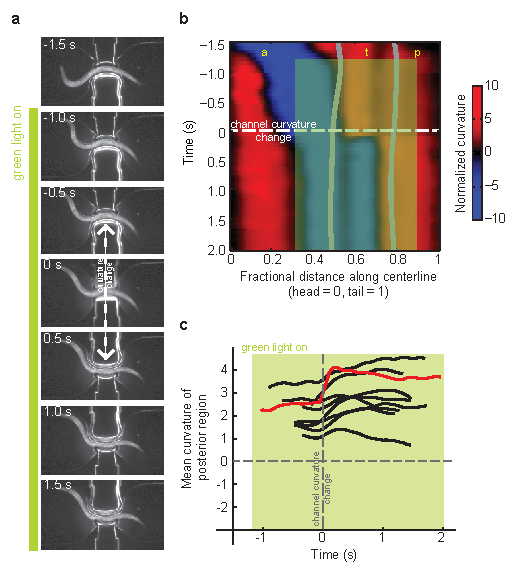
\includegraphics[width=0.87\textwidth]{figures/proc4}
\caption[ Optogenetic inactivation of cholinergic motor neurons.] { Optogenetic inactivation of cholinergic motor neurons.   
(\textbf{a}) Video images of a transgenic worm (P\textit{unc17::NpHR}) partially trapped in a pneumatic 
microfluidic channel. Green bar indicates the duration of green light illumination of the middle 
portion of the worm before and after induced change in channel curvature at $t = 0$ s. As a result, 
the curvature of the tail failed to follow the curvature change of the channel (also see 
Supplementary Movie 8). 
(\textbf{b}) Curvature kymograph of the transgenic worm trapped in the channel as shown in (\textbf{a}). Green 
shading indicates the body region and duration of green light illumination. 
(\textbf{c}) Curvature of the posterior body region, measured as an average from the posterior limit of the 
channel to the tail, during onset of illumination (green shading) and the induced change in 
curvature of the middle region at $t = 0$ (dashed line). Representative data from five worms were 
shown. Red curve corresponds to the experiment shown in (\textbf{a}) and (\textbf{b}). 
\label{fig:proc4}}
\end{figure}

Next, we studied \textit{vab-7} mutants, whose dorsal B-type cholinergic motor neurons (DB) reverse 
the direction of their processes \citep{esmaeili_c._2002}. During unrestrained forward movement, the bending wave 
in the anterior of \textit{vab-7} mutants exhibits both dorsal and ventral curvatures whereas the bending 
wave that propagates to posterior regions exhibits only ventral curvatures (Supplementary Fig. 
3a, c-d and Supplementary Movie 9). In other words, only ventral bending waves propagate 
through the worm body. When we trapped \textit{vab-7} mutants in the pneumatic microfluidic device, 
we found that the posterior region of the worm was unable to follow the bending of the channel 
to the dorsal side (Supplementary Fig. 3b, e-f and Supplementary Movie 10). Taken together, 
these results suggest that the B-type cholinergic motor neurons are required to close a 
proprioceptive feedback loop that drives the bending signal along the motor circuit during 
forward movement. 


\subsection{Body wall muscles exhibit hysteresis}
 
Deactivating cholinergic motor neurons in transgenic worms (P\textit{unc17::NpHR}) locked the worm 
in the whatever bending posture the worm had adopted immediately preceding illumination (Fig. ~\ref{fig:proc4} and  \citep{leifer_optogenetic_2011}). We thus ask 
whether \textit{C. elegans} muscles could sustain contraction even in the absence of motor neuron inputs. 
To test this possibility, we optogenetically stimulated body segments in transgenic worms (P\textit{myo- 3::ChR2}) expressing Channelrhodopsin-2 in body wall muscles while abolishing motor neuron 
inputs. To abolish motor neuron inputs, we treated transgenic worms with ivermectin, which 
hyperpolarizes the motor circuit by activating glutamate gated chloride channel \citep{dent_genetics_2000,cully_cloning_1994}, but 
does not directly affect muscle cells \citep{hart_behavior_2006}. When we optogenetically induced body bending in 
paralyzed worms, the bend would persist long after turning off the illumination (Supplementary 
Fig. 4a-b and Supplementary Movie 11). The bend would gradually relax over \textasciitilde40 s, but often in 
a series of abrupt jumps (Supplementary Fig. 4c). We observed similar phenomenon when 
ivermectin treated worms are in the \textit{unc-13(s69)} background (Supplementary Movie 12), a loss 
of function mutation that abolishes synaptic transmission from both GABAergic and cholinergic 
motor neurons to muscles \citep{richmond_unc-13_1999}. Taken together, these results suggest that \textit{C. elegans} body wall 
muscles indeed exhibit a form of hysteresis; they can maintain stable levels of contraction long after stimulation.  

\section{Discussion}
Russell and Byerly noted that the cholinergic motor neurons have long and synapse free 
processes that extend along the ventral and dorsal nerve cords, and speculated that these 
processes might represent stretch-sensitive antennae to detect changes in body posture (cited in 
 \citep{white_structure_1986,chen_neuronal_2007} and Supplementary Fig. 1b). In theoretical models of the worm motor circuit, 
Niebur and Erdos \citep{niebur_theory_1991} used proprioceptive coupling hypotheses as a mechanism to propagate 
bending signals. Here, we have shown that the cholinergic motor neurons are required to 
transduce stretch-sensitive signals, and that this form of proprioceptive coupling represents a key 
mechanism for propagating bending signals along the \textit{C. elegans} body during forward 
locomotion. Posterior body segments are compelled to bend in the same direction as anterior 
segments through stretch-sensitive signals transduced by the cholinergic motor neurons. 
Proprioceptive coupling could explain the organization of the undulatory gait without the need to 
invoke ensembles of center pattern generators (CPG) along the motor circuit, like body segments 
in lamprey and leech are thought to behave \citep{ermentrout_frequency_1984}.  
 
The small size and experimental accessibility of the \textit{C. elegans} motor circuit suggest that it might 
be possible to build computational models of locomotion that integrate the dynamics of all 
neuronal and muscle components. Our results suggest that any computational framework for the 
\textit{C. elegans} locomotory circuit must integrate the biomechanics of undulatory movement itself 
with neuromuscular activity. In \textit{C. elegans}, the motor circuit organizes the undulatory gait for forward locomotion by both detecting and driving bending activity.




\section{Manuscript Information}
\subsection{Submitted for publication as}
A previous version of this chapter was submitted as \citep{wen_bending_2011}:

\bibentry{wen_bending_2011}

\subsection{The Author's Contribution}
The overwhelming majority of the work in this chapter was performed by Quan Wen. Andrew M.~Leifer assisted with optogenetic experiments and provided technical support regarding instrumentation and experimental design. Additionally, Andrew made major contributions to the analysis software. 

The majority of the manuscript was written by Quan Wen and Aravinthan D.T.~Samuel.
